\documentclass{article}
\usepackage{graphicx,fancyhdr,amsmath,amssymb,amsthm,subfig,url,hyperref}
\usepackage[margin=1in]{geometry}
\usepackage{xltxtra}
\usepackage{xgreek}
\usepackage{amsfonts}
\usepackage{amssymb}
\usepackage{amsmath}
%\setmainfont[Mapping=tex-text]{Times New Roman}
\setmainfont{GFS Artemisia}
%----------------------- Macros and Definitions --------------------------

% FILL THIS OUT
\newcommand{\studentname}{Νικόλαος Ζαρίφης}
\newcommand{\suid}{03112178}
\newcommand{\exerciseset}{Πρώτη εργαστηριακή Άσκηση}
% END



\renewcommand{\theenumi}{\bf \Alph{enumi}}

%\theoremstyle{plain}
%\newtheorem{theorem}{Theorem}
%\newtheorem{lemma}[theorem]{Lemma}

\fancypagestyle{plain}{}
\pagestyle{fancy}
\fancyhf{}
\fancyhead[RO,LE]{\bfseries\large NTUAthens}
\fancyhead[LO,RE]{\bfseries\large Δίκτυα επικοινωνιών}
\fancyfoot[LO,RE]{\bfseries\large \studentname: nick.zarifis@hotmail.com}
\fancyfoot[RO,LE]{\bfseries\thepage}
\renewcommand{\headrulewidth}{1pt}
\renewcommand{\footrulewidth}{1pt}

\graphicspath{{figures/}}

%-------------------------------- Title ----------------------------------

\title{Δίκτυα επικοινωνιών \\ \exerciseset}
\author{\studentname \qquad  ID: \suid}

%--------------------------------- Text ----------------------------------

\begin{document}
\maketitle

\section*{Problem 1}
\begin{enumerate}
\item %A
Για να βρούμε τον ρυθμό μετάδωσεις έχουμε ότι στέλνουμε
$1000B/0.005s$ το οποίο συνεπάγεται $\frac{8*1000}{0.005}bits/s \rightarrow 2^4*10^5bits/s$
\item
Στέλνουμε πακέτα για 6s και στέλνουμε ένα πακέτο ανα 0.005s. Άρα έχουμε :$6/0.005 =1200packets \rightarrow 1200*packets\ bits \rightarrow 12*10^5 bytes \rightarrow 
9.6*10^6 bits/s$ . Βλέπουμε ότι συμφωνεί με το αποτέλεσμα του προηγούμενου ερωτήματος.
\item 
Αφού ψάχνουμε την γενική περιπτώσει θα μετρήσουμε την στιγμή που θα φτάσει το πρώτο bit στο τερματικό κόμβο.
Έχουμε καθηστέριση 10ms άρα ενα bit θέλει 10ms να φτάσει στο τέρμα. Έχουμε λοιπόν,$10*0.001/0.005=2 packets$ άρα στην γραμμή θα υπάρχουν συνχρόνος μέγεθος πληροφορίας 2 πακέτων.Έχουμε λοιπόν 2000B.Το animation φυσικά μας δίνει το ίδιο αποτελεσμά ακριβώς.
\item 
Από τον παραπάνω τύπο βλέπουμε ότι η καθηστέρηση είναι ανάλογη των πακέτων άρα θα έχουμε 4 πακέτα οπότε 4000Β.
\item
Άμεσα απο το πρώτο ερώτημα βλέπουμε ότι το αποτέλεσμα είναι $\frac{960 *8}{0.005}=1536000 bits/s$
\item
Ο ρυθμός μεταδώσεις μεταβάλετε αναλογικά με τον ρυθμό μεταδώσεις των πακέτων  [εντολή: set interval\_ RATE  ] και ανάλογα με το μέγεθος του πακέτου [εντολή: set packetSize\_ SIZE].
\item
Άλλαζοντας το μέγεθος πακέτου πρώτα: $1,2 * 10^6=\frac{8*\text{Size}}{0.005}\rightarrow \text{Size}=0.75 *10^3=750B$ Άρα: $790Β \rightarrow 1.264MBps$ δεν ξεπερνάμε την γραμμή .Αλλάζωντας το rate έχουμε: $1,2 * 10^6=\frac{8*1000}{\text{rate}}\rightarrow \text{rate}=\frac{1}{0.15*10^3}=6.6 ms$. Βλέπουμε πάλι οτι $\frac{8*1000}{0.0066}=1.212MBps$Άρα ακόμα δεν ξεπερνάμε το όριο.
\item
Για να μην έχουμε απώλεια θα πρέπει το Rate<2Mbps. Άρα έχουμε δυο περιπτώσεις , 1. Αυξάνοντας το packet size βλέπουμε ότι το μέγιστο είναι $2*5*10^3/8 =1250B $ . Μεταβάλλοντας το interval βλέπουμε ότι η οριακή συνθήκη είναι $\frac{8000}{2*10^6}=4ms$
\end{enumerate}

\section*{Problem 2}
\begin{enumerate}
\item %A
Παρατηρούμε ότι αν αυξήσουμε το packet size παραπάνω απο το μέγιστο η γραφηκη παράσταση αρχίζει να γινεται τριγωνική γιατί χάνονται πακέτα (γινεται ψαλιδισμός). 
\\
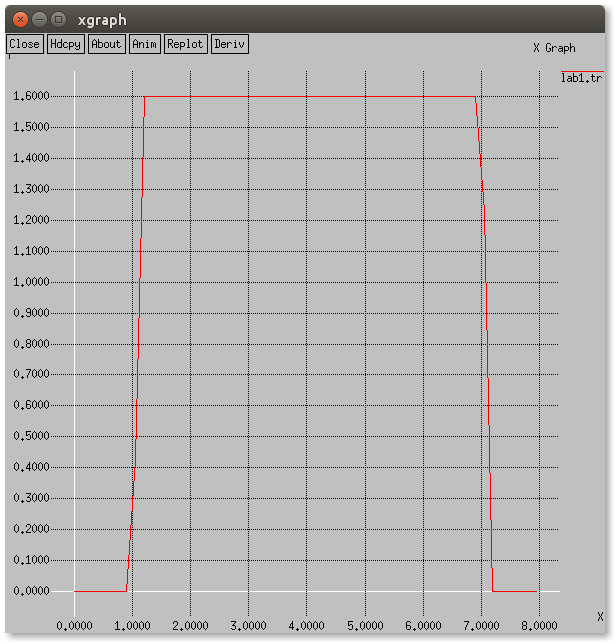
\includegraphics[witdh=200,height=200]{xgraph1.png} \
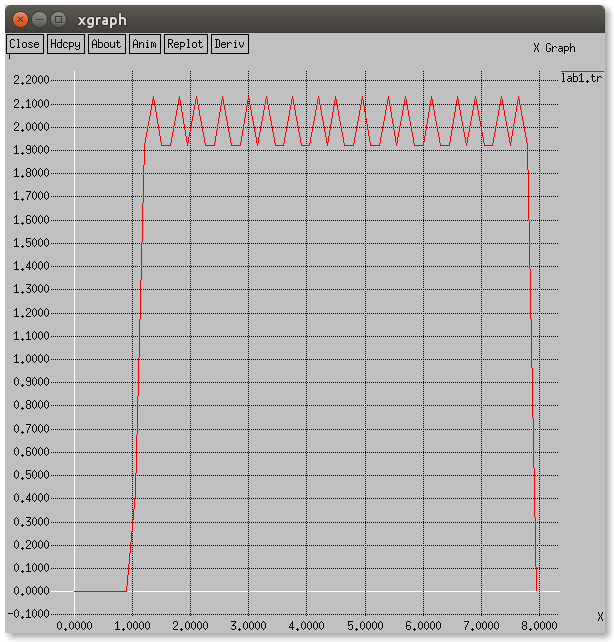
\includegraphics[witdh=200,height=200]{xgraph2000.png}
\item
Όπως έχουμε αποδείξει ήδη το μέγιστο μήκος είναι 1250B.(βλ. παρακάτω εικόνα). Αν αυξήσουμε λίγο παραπάνω βλέπουμε πάλι ψαλιδισμό. \\
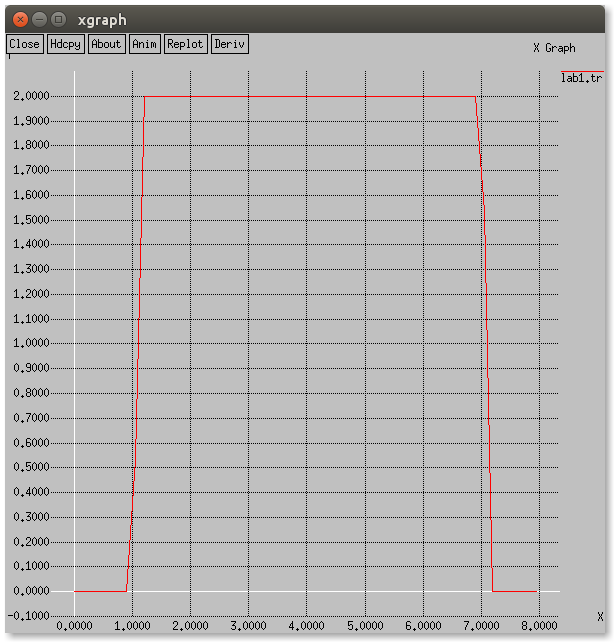
\includegraphics[witdh=200,height=200]{xgraph1250.png}
\item
Αυξάνοντας και μειώνοντας  το interval  μείνουμε κι αυξάνουμε αντίστοιχα τον ρυθμό μετάδοσης, έτσι όταν ξεπεράσουμε την χωρητικότητα της γραμμής παρατηρήτε ψαλίδισμα.
\\
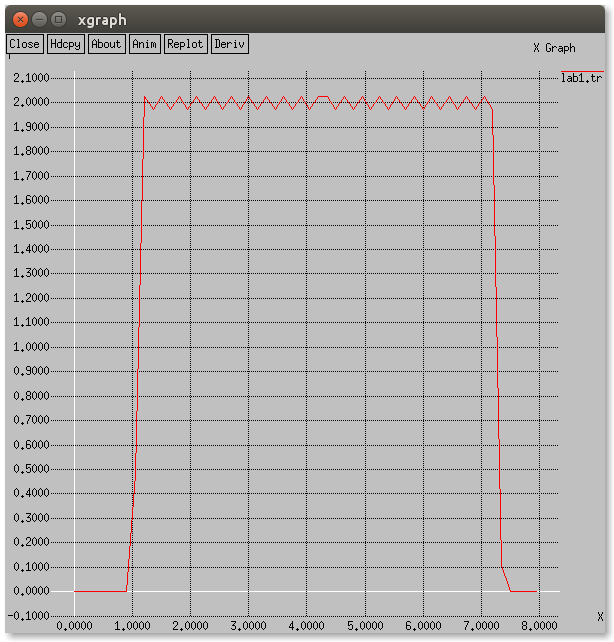
\includegraphics[witdh=200,height=200]{xgraph0005.png} \ 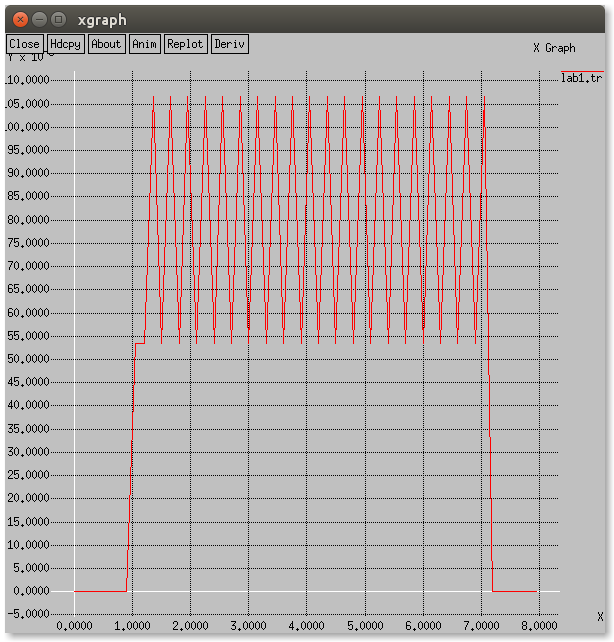
\includegraphics[witdh=200,height=200]{xgraph01.png}
\item
Βλέπουμε πως η γραφική πήγε 0.5s πιο δεξιά πράγμα που συμβαίνει γιατί η γραφική σχεδιάζεται σύμφωνα με τον υποδοχέα ο οποίος έχει μεγαλύτερη καθυστέρηση στο να πάρει τα πακέτα.
\\
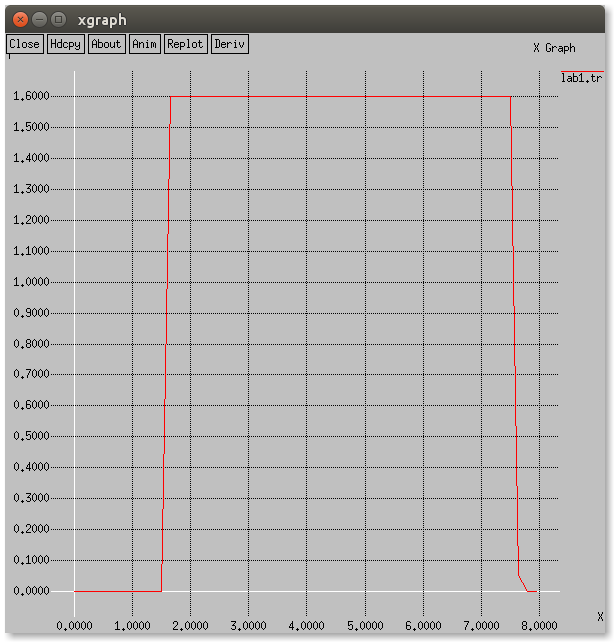
\includegraphics[witdh=200,height=200]{xgraphms.png}
\item
Κάνοντας πιο αργό το record βλέπουμε πως αργεί περισσότερο να πάρει δείγμα με αποτέλεσμα να έχουμε μια  παράσταση όπως θα ήταν η μέση κίνηση.\\ 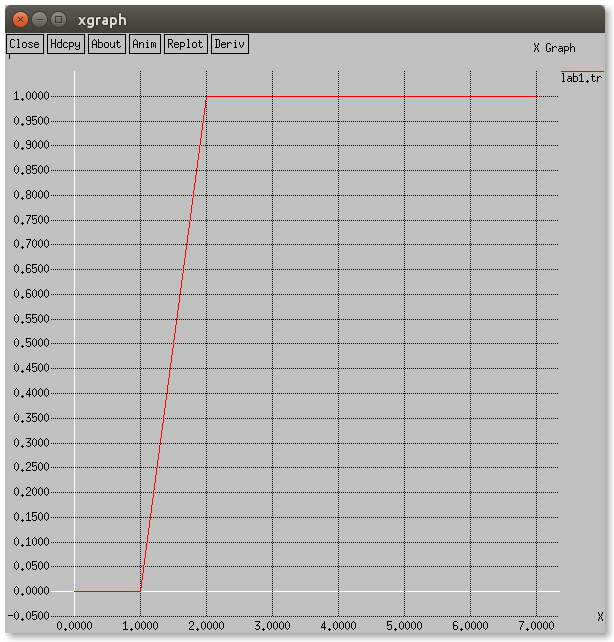
\includegraphics[witdh=200,height=200]{1s.png} \\
Αντίστροφα αυξάνοντας το record βλέπουμε πως η παράσταση μοιάζει με τετραγωνικό παλμό πράγμα λογικό αυτό μας κάνει για την στιγμιαία κίνηση.
\\ 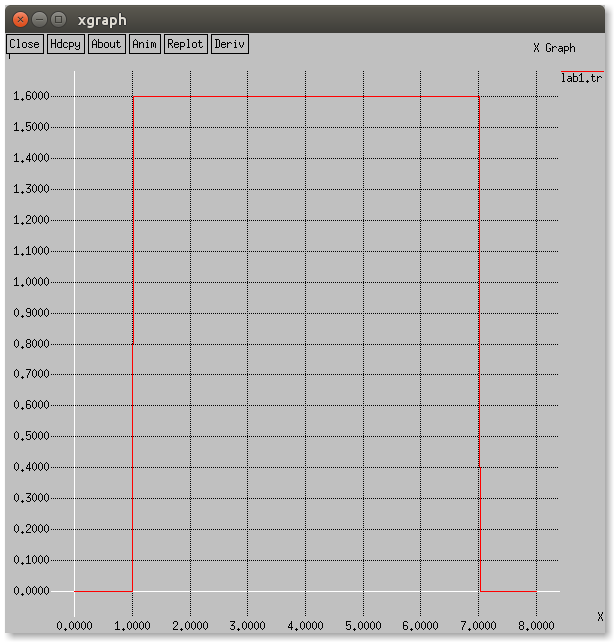
\includegraphics[witdh=200,height=170]{001.png}
\item
Έχοντας αλλάξει σε expomental , αυτό συμβαίνει γιατί οι χρόνοι των περιόδων που γενιούνται τα πακέτα προέρχονται απο εκθετικές κατανομες σε αντίθεση με πριν που ήταν σταθερές. 
\\ 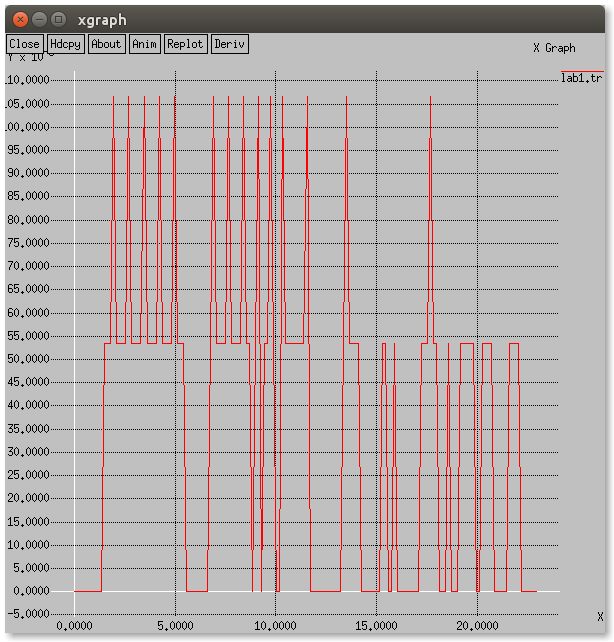
\includegraphics[witdh=200,height=170]{exp.png}
\end{enumerate}


\end{document}
